\documentclass[12pt]{article}
\usepackage[margin=1in]{geometry}
\usepackage{enumerate}
\usepackage{graphicx}


\title{EECS 314 - Project Report}
\author{Haley Eisenshtadt, Jason Kuster, Ian Lavelle, Joseph Satterfield, James Wright}

\begin{document}
	\maketitle
	\section{Problem Statement}
	While learning MIPS in EECS 314, our group noticed a lack of fun, interactive tools to make learning MIPS easier. There are helpful demonstrations in the textbook and you can always open up QtSpim and play around, but there wasn't anything particularly graphical and interactive to help people learn MIPS. Our group wanted to put together an Android app to make the process of learning MIPS easier. The tool we settled on to build this was Unity, a cross-platform game engine which several of us had used before which made game development easy.
	\section{Major Challenges}
	There were a couple of challenges we ran up against while developing this set of games.
	% Put some major challenges we ran up against here. Format is \item <PUT TEXT HERE>
	\begin{enumerate}
		\item Item 1
		\item 
	\end{enumerate}
	\section{Key Components}
	Our project has three key components which come together to make the MIPS learning process easier. We have the MIPS Learner, which is a graphical MIPS simulator in the style of ALICE for Java, we have MIPS Bejeweled, a twist on the classic Bejeweled game which helps teach people how MIPS instructions work, and we have the Pipeline Bakery which presents the MIPS pipeline in a fun, graphical way.
	\subsection{MIPS Learner}
	\subsection{MIPS Bejeweled}
	\subsection{Pipeline Bakery}
	\section{Integration}
	\section{User Interface}
	\section{Snapshots}
	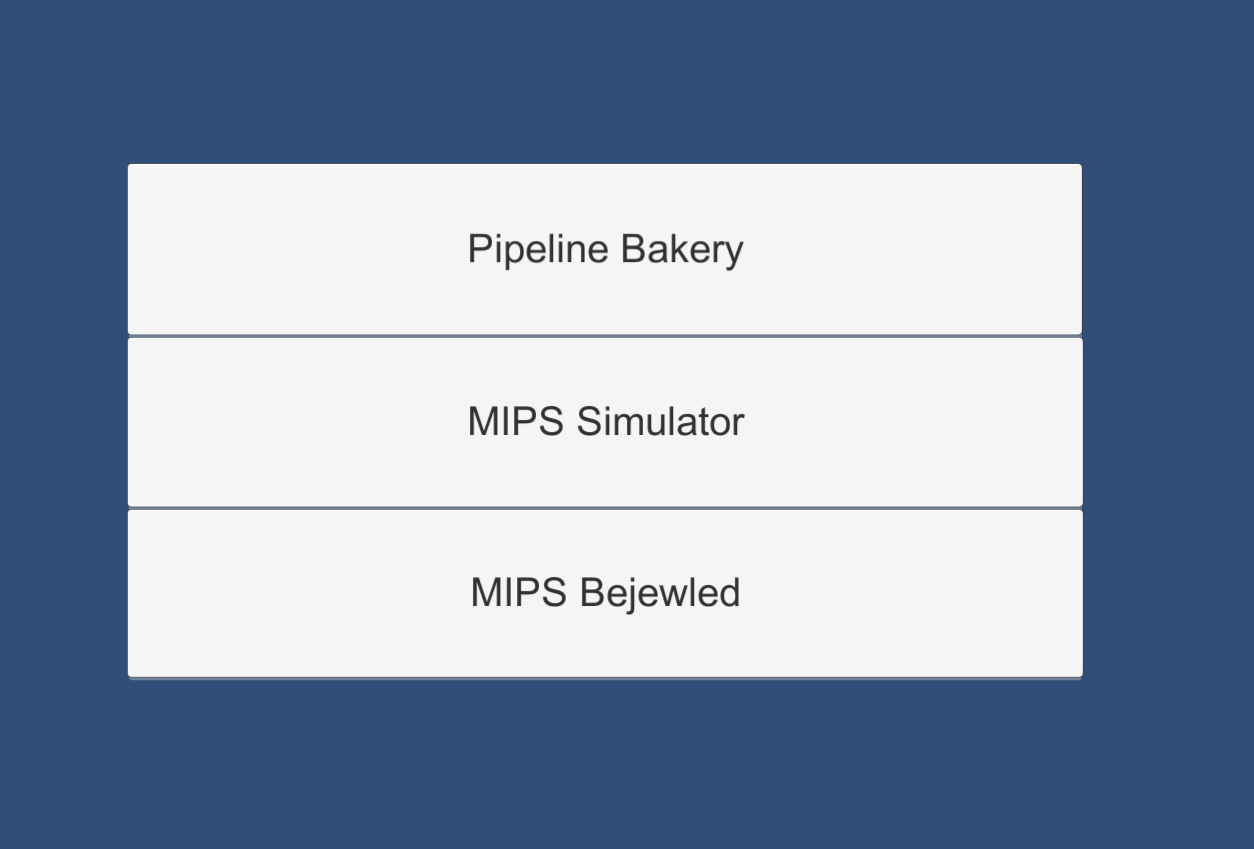
\includegraphics[height=8cm]{MainMenu.png}\\
	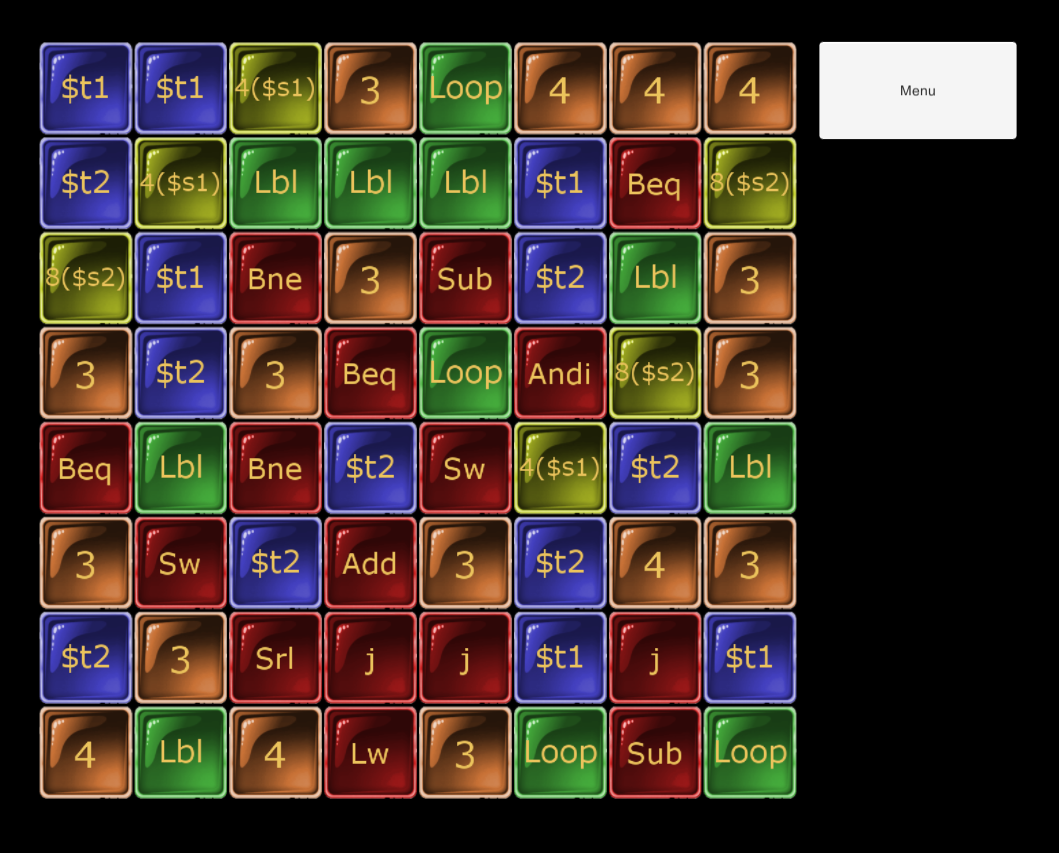
\includegraphics[height=6cm]{MIPSBejeweled.png}
	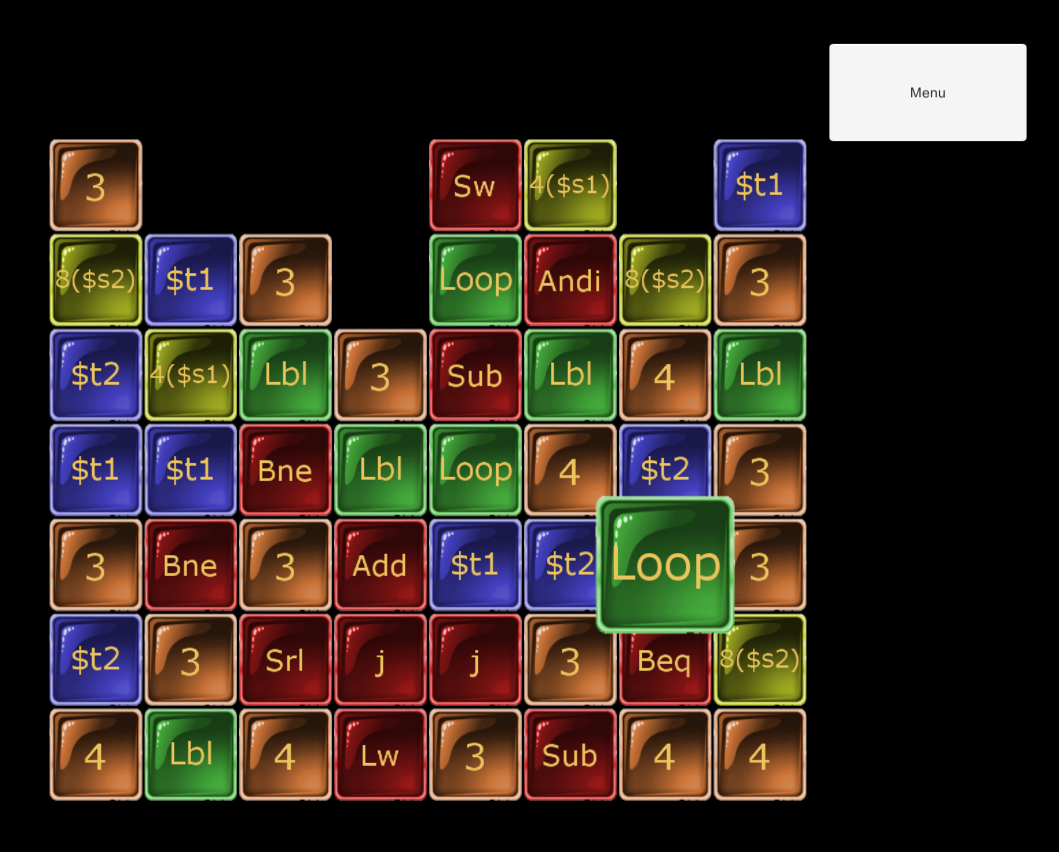
\includegraphics[height=6cm]{BejeweledHowTo.png}\\
	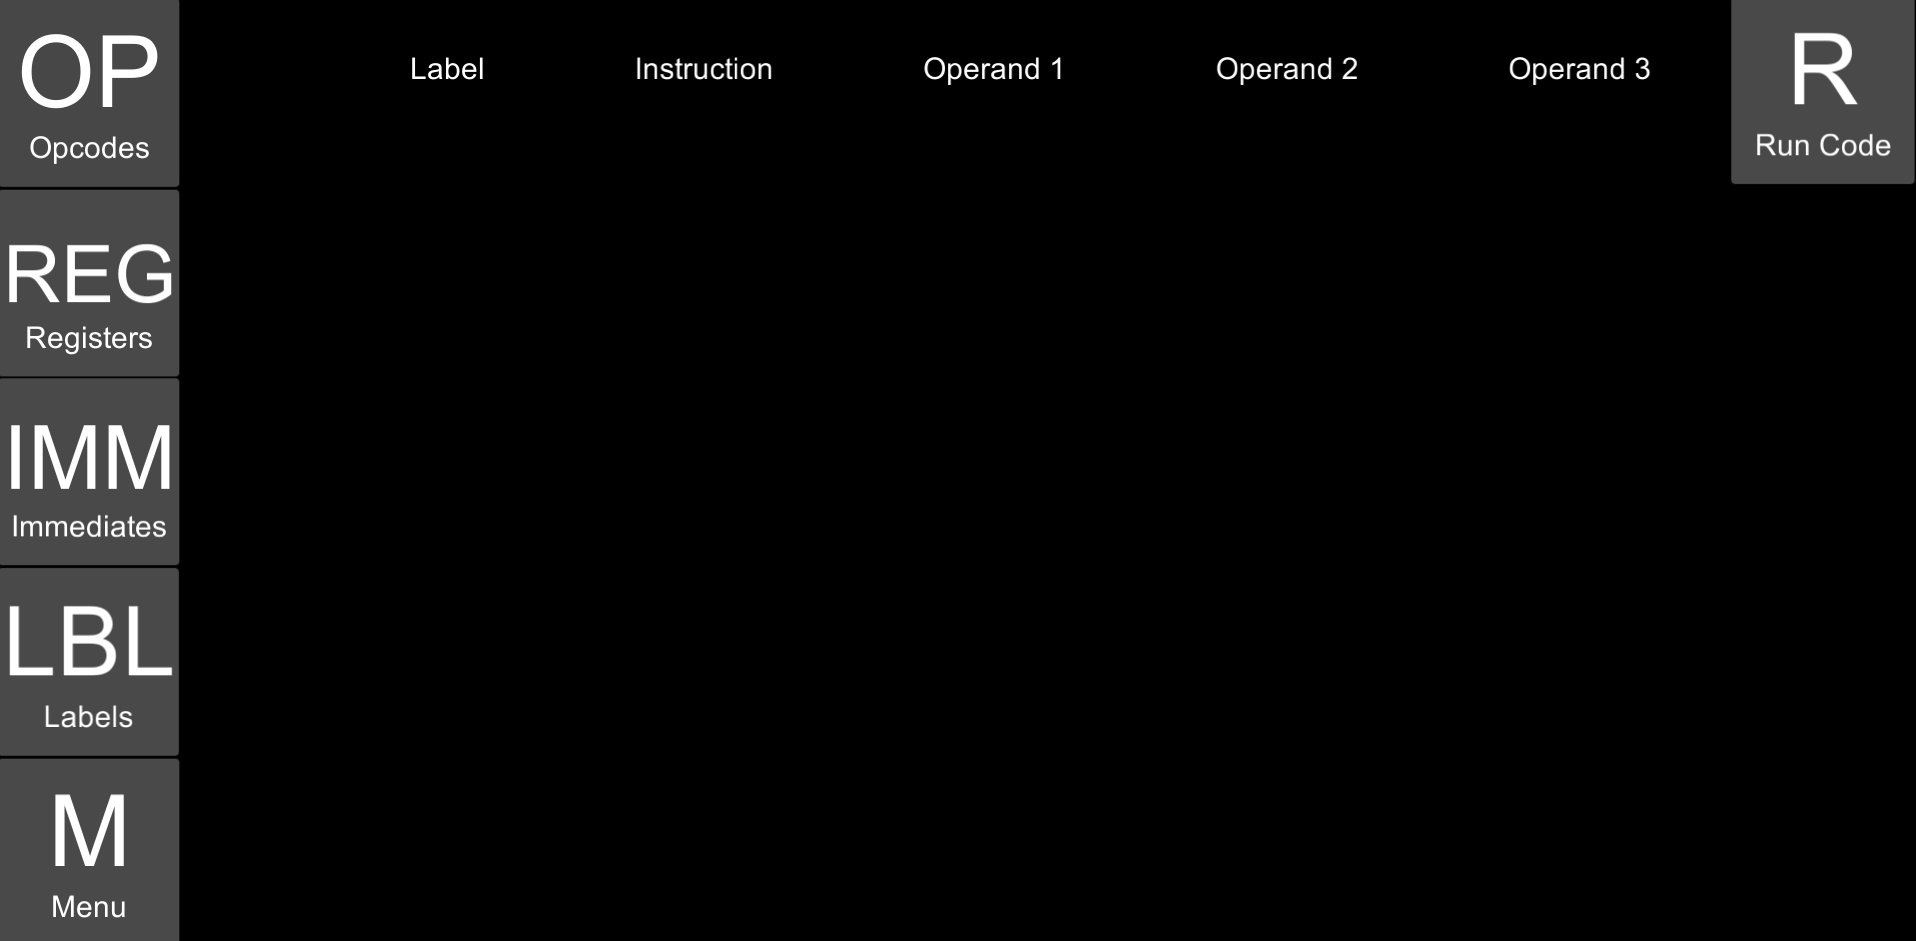
\includegraphics[height=4cm]{MIPSSimulatorStart.png}
	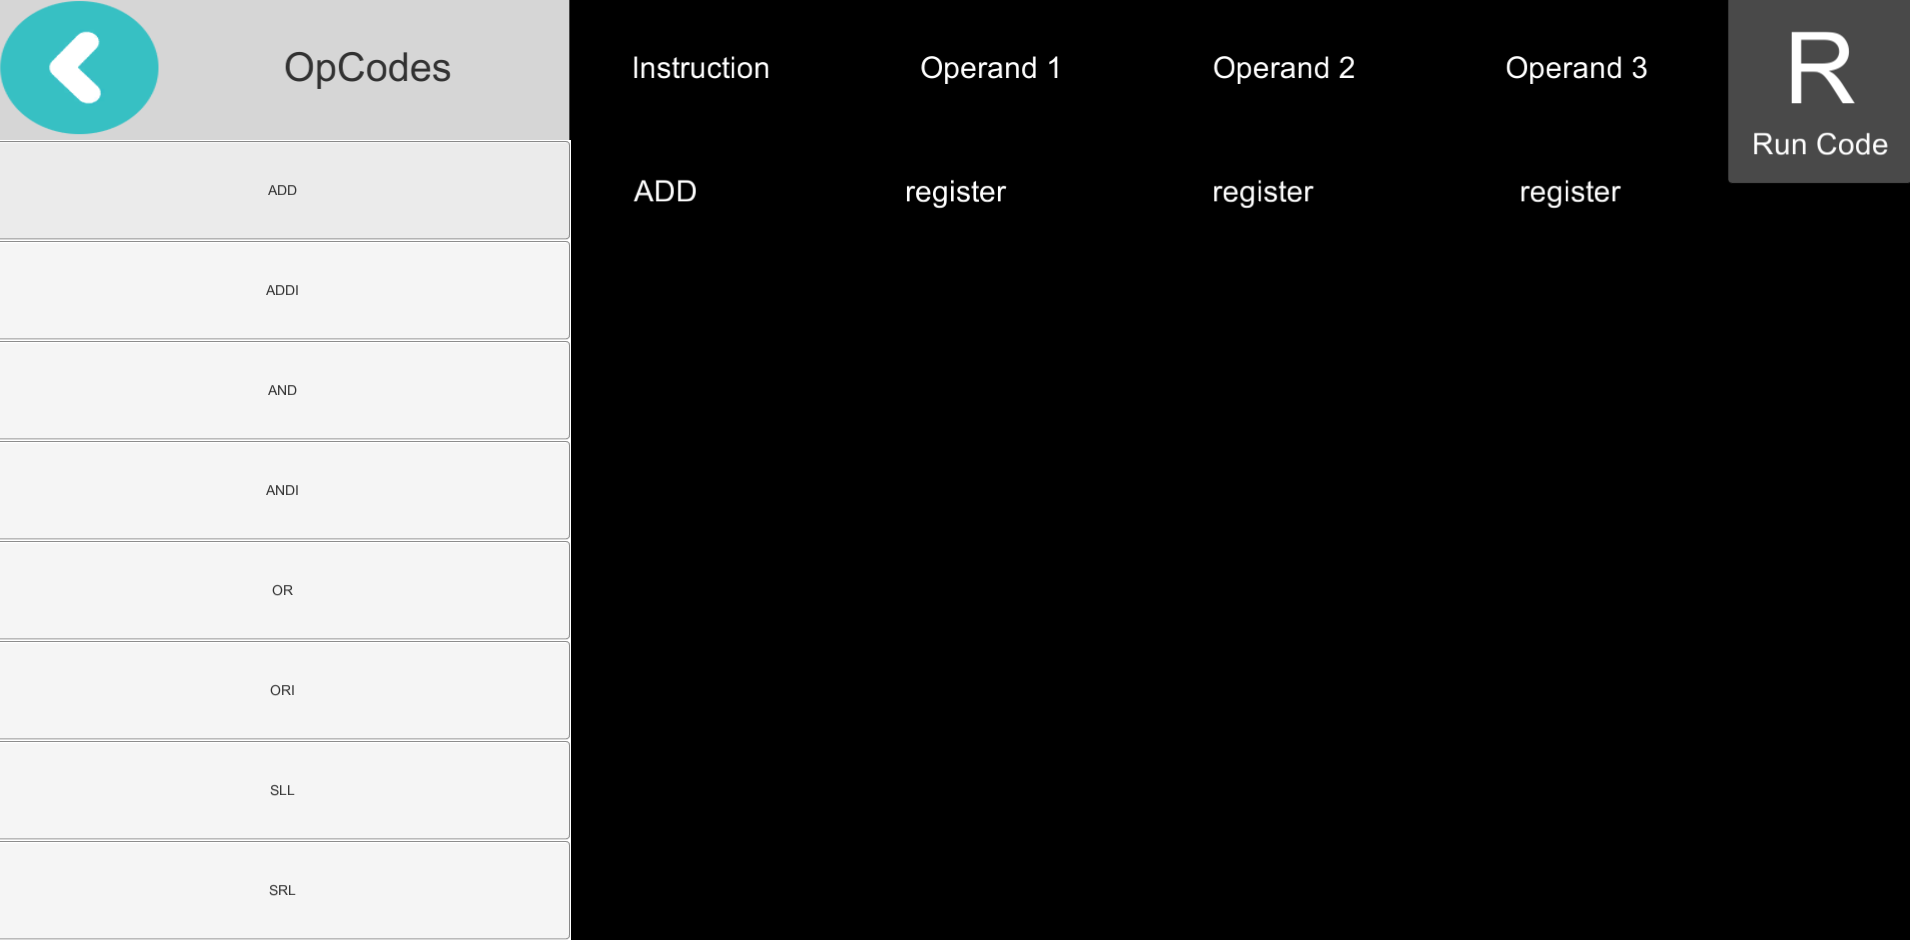
\includegraphics[height=4cm]{MIPSSimulatorProgress.png}\\
	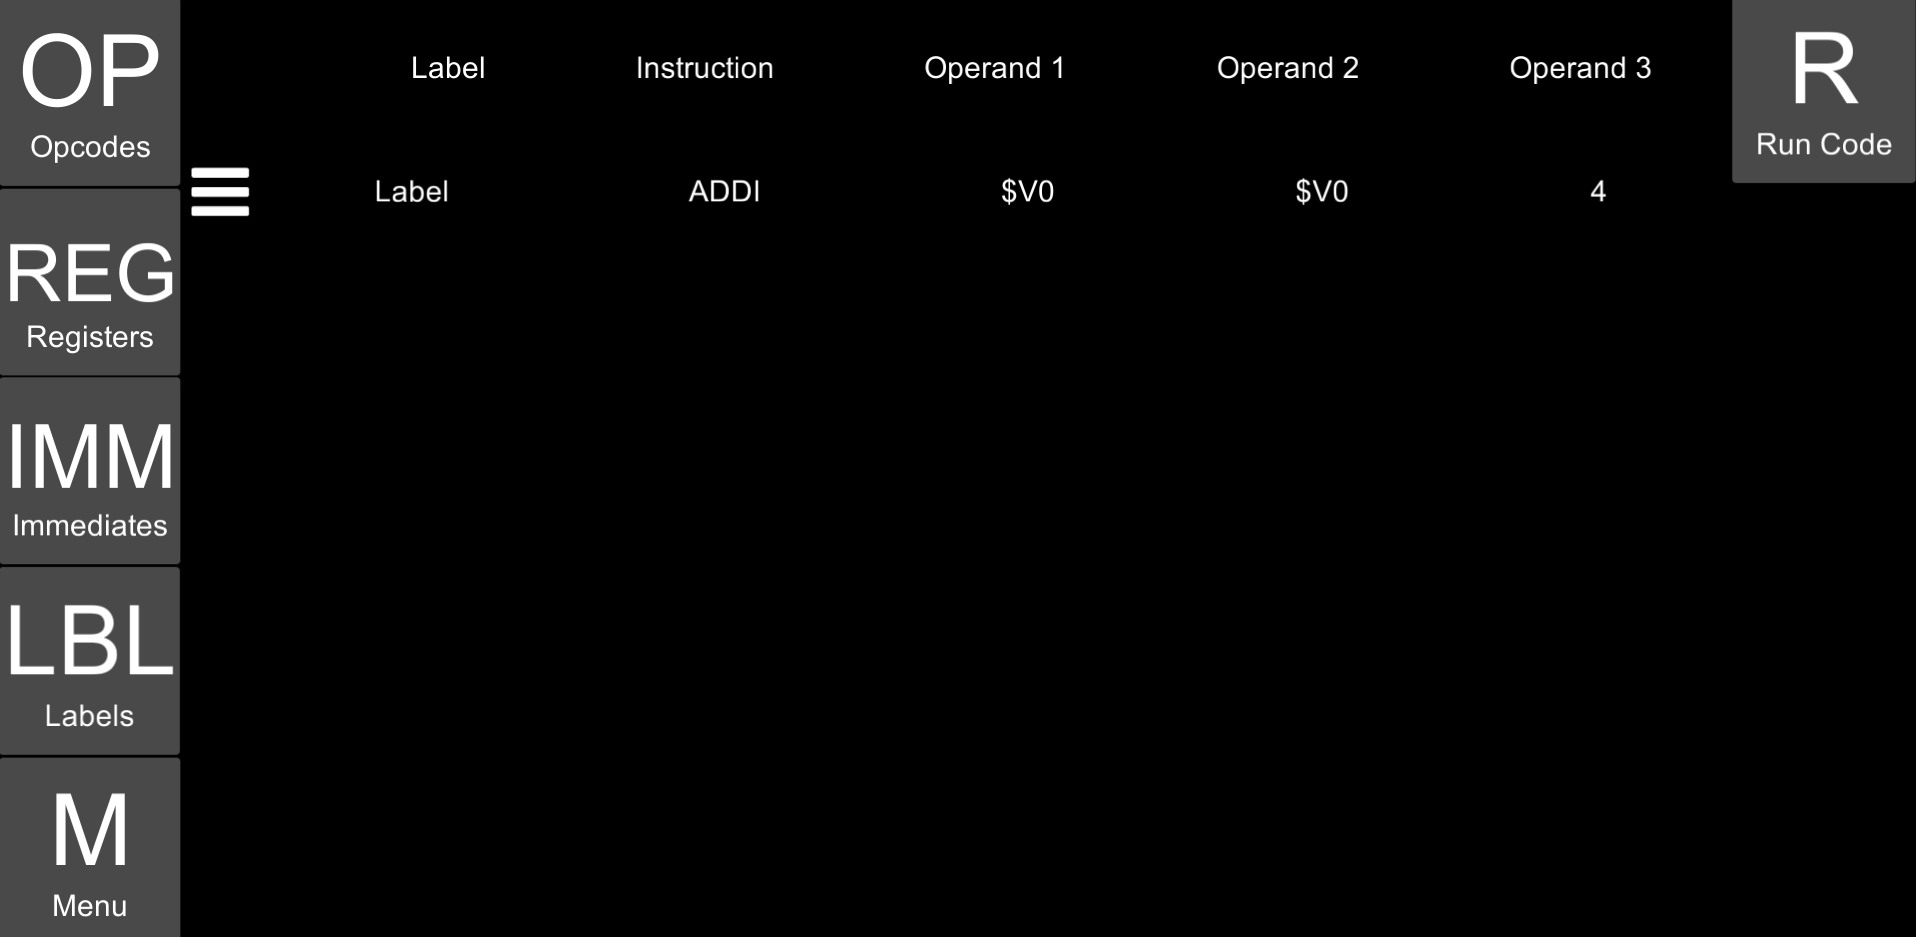
\includegraphics[height=4cm]{MIPSSimulatorReady.png}
	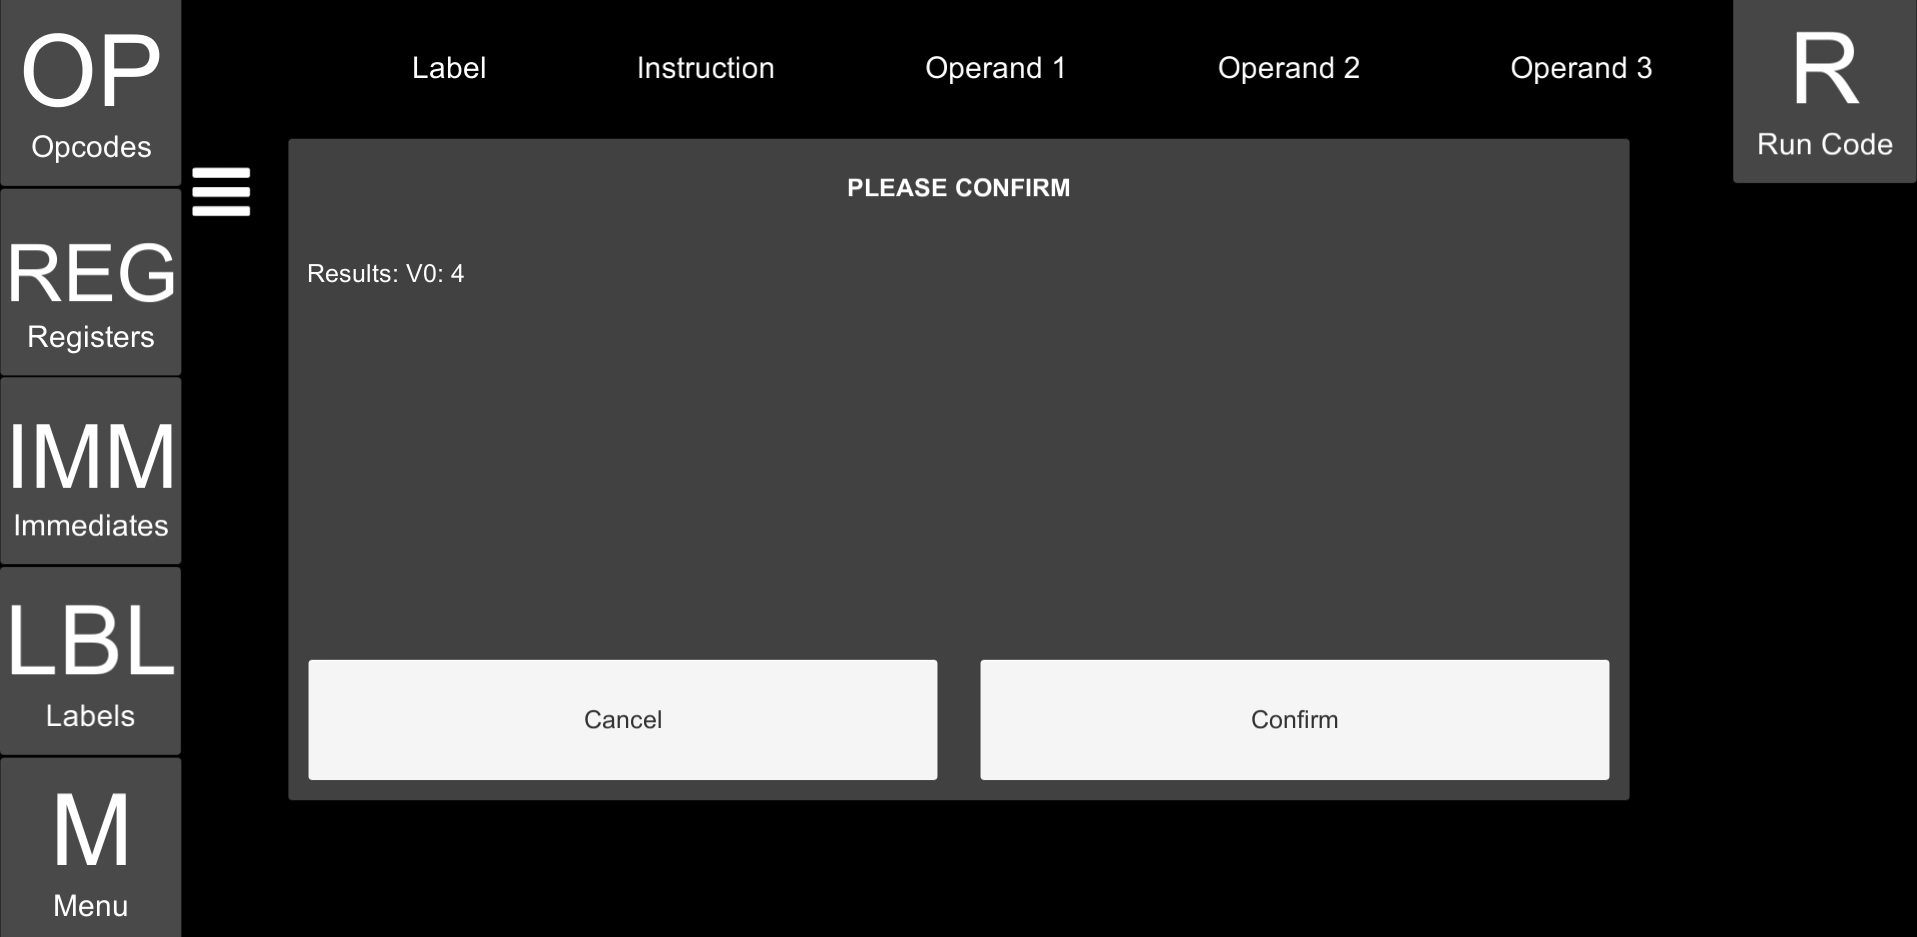
\includegraphics[height=4cm]{MIPSSimulatorRun.png}\\
	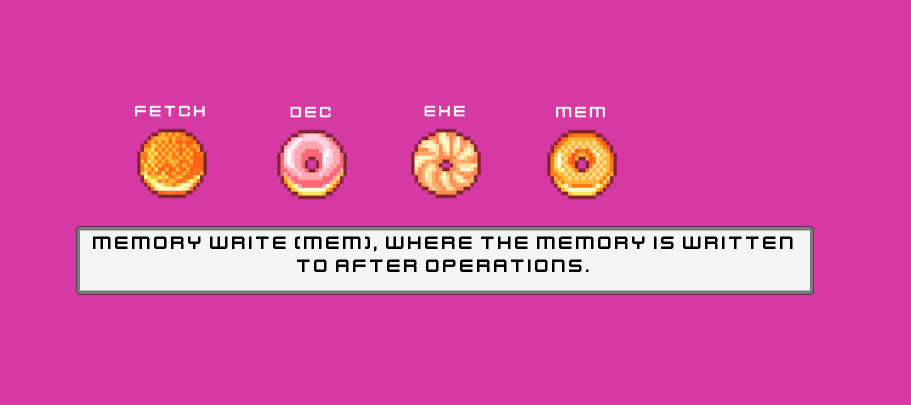
\includegraphics[height=4cm]{PipelineBakeryTut.png}
	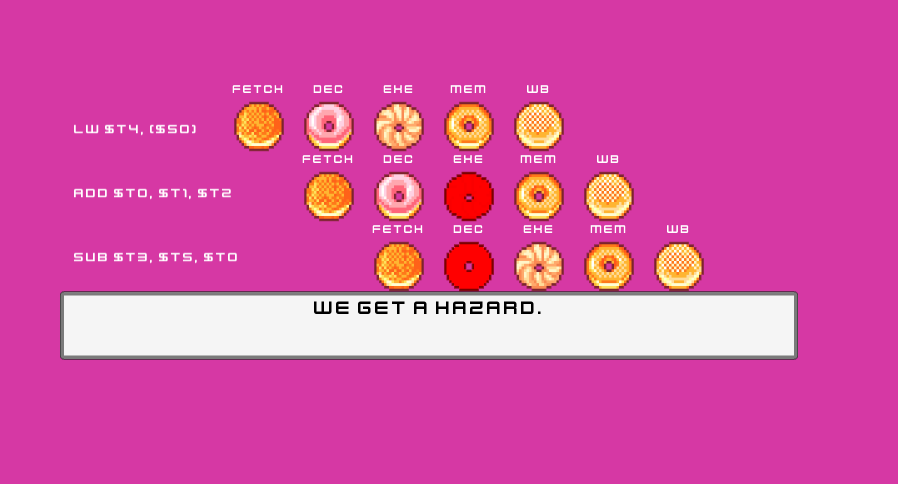
\includegraphics[height=4cm]{PipelineBakeryTut2.png}\\
	\section{Individual Contributions}
	\begin{itemize}
		\item Haley Eisenshtadt
		\subitem Pipeline Bakery Design/Implementation
		\item Jason Kuster
		\subitem Bejeweled Block Physics
		\subitem Project Report Lead
		\subitem Project Report Compilation
		\item Ian Lavelle
		\subitem Bejeweled Base Implementation
		\subitem Bejeweled Instruction Logic
		\item Joe Satterfield
		\subitem MIPS Learner Implementation
		\item James Wright
		\subitem MIPS Learner Implementation
	\end{itemize}
\end{document}